\section{System Design} % talk about general blackboard system structure

A Blackboard System is a way for distinct agents specializing in subproblems to communicate partial solutions and cooperate to find a complete solution.
There are three components of a Blackboard System: the Blackboard, the Control, and the Knowledge Sources.
Knowledge Sources are the specialized agents. They examine the Blackboard as input and write their partial solutions on the Blackboard.
The Blackboard is a data structure shared by all the Knowledge Sources and presided over by the Control. It is essentially an open read and write area.
The Control decides which Knowledge Sources run and when the problem has been solved.

\begin{figure}[h]
\caption{Structure of a general blackboard system}
\centering
	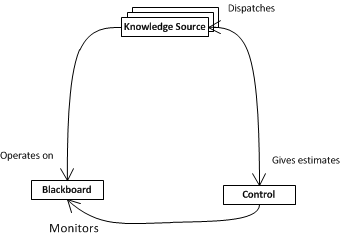
\includegraphics[keepaspectratio=true]{blackboard-system-diagram.png}
\end{figure}

\subsection{Blackboard} % talk about the specific blackboard used

For this music composition system, the Blackboard contains two major items: the given musical line, the \emph{cantus firmus}, and the musical line in the progress of composition, the \emph{counterpoint}.
The \emph{cantus firmus} is a read only list of notes along with a note-at-time lookup table for fast random access.
The \emph{counterpoint} is also a list of notes, but Knowledge Sources are allowed to extend or modify it.
Both provide a context-aware location reference (known as a Zipper) that makes it easier for Knowledge Sources and the Control to communicate about particular areas of a composition.
The Blackboard also contains other minor, but important, information such as the key or mode of the composition. This is mainly for ease of reference.
An important aspect of the Blackboard is that it is immutable, a side effect of using Haskell as the implementation language.
This is actually very useful because if a potential composition runs into a dead end, previous versions of the Blackboard are still around, making backtracking trivial.

% TODO insert a diagram of the blackboard structure?

\subsection{Knowledge Sources} % talk about the general structure for agents

Knowledge Sources, or agents, embody musical rules or preferences and can range from simple to complex.
Most of Counterpoint is specified by either forbidding certain kinds of musical structures or limit their use so that others are preferred.
These are respectively known as `hard' and `soft' rules. Ideally, the system should know violate any hard rules and minimized violations of soft rules.
Agents embodying these rules essentially examine a location in a musical line and test whether their rule is upheld or not.
These agents exist to cut off the composition when it progresses in an undesirable way.

The counterpart to these tester agents are agents that modify the composition by extending it or changing an existing portion.
The most basic version of this type of agent just attaches random notes, within the allowed range, to the end of the existing composition.
More complex agents could make sweeping modifications to achieve higher level musical constructs, such as tension and contour.

\subsection{Control} % talk about the control structure

The Control keeps a task queue of modified locations in the \emph{counterpoint} line.
These locations are ordered by length into the line and by number of and severity of rule violations.
The result is that locations farther into the composition and with fewer violations are at the front of the queue.
These provide the most promise of completing the composition, so the system focuses on them.
Locations without rule violations are prefered even if they are not as far along.
If no clean positions are left, the system will try to break as few soft rules as necessary.

The Control dispatches test agents to newly generated locations and dispatches generating agents to throughly tested locations.
This encourages progress along successful compositional paths, while allowing for experimentation and backtracking if necessary.
Control terminates the composition when it finds a valid \emph{counterpoint} that is the same length as the \emph{cantus firmus}.
